\chapter{Dataset and Exploratory Data Analysis}\label{chap:donnees}

\section{Introduction}
A classifier can only be as reliable as the data it learns from. Before any model is trained, this chapter describes the firewall log used in the project, audits its quality, and explores how the traffic features relate to the action taken by the firewall. The exploration has two goals: to understand the structure of the problem (which features separate the actions, which ones are redundant), and to identify the risks that the experimental protocol of Chapter~\ref{chap:methodologie} must control, in particular class imbalance, duplicated records and possible target leakage. The descriptive results come from \texttt{notebooks/01\_eda\_and\_cleaning.ipynb}; the statistical tests come from \texttt{notebooks/07\_statistical\_tests.ipynb}.

\section{Dataset Source and Description}
The data set is the \emph{Internet Firewall Data} published in the \ac{UCI} Machine Learning Repository (data set \#542)~\cite{dua2019uci}. It contains \textbf{65\,532 records} logged by the firewall of a single organisation. Each record describes one network flow by \textbf{eleven numerical attributes} and the \textbf{action} that the firewall applied to it, which is the target variable. Table~\ref{tab:attributs} describes the twelve columns. The file \texttt{data/raw/log2.csv} (2.9~MB) contains no missing value.

\begin{table}[htbp]
  \centering
  \caption{Description of the twelve columns of the data set}
  \label{tab:attributs}
  \small
  \begin{tabular}{|l|p{5.6cm}|l|r|}
    \hline
    \textbf{Attribute} & \textbf{Meaning} & \textbf{Nature} & \textbf{Distinct values} \\
    \hline
    Source Port & Port of the client that opened the flow & identifier & 22\,724 \\
    Destination Port & Port of the requested service (e.g.\ 53 = DNS, 443 = HTTPS) & identifier & 3\,273 \\
    NAT Source Port & Source port after \ac{NAT} (0 = no translation) & identifier & 29\,152 \\
    NAT Destination Port & Destination port after \ac{NAT} & identifier & 2\,533 \\
    Bytes & Total bytes exchanged & count & 10\,724 \\
    Bytes Sent & Bytes sent by the source & count & 6\,683 \\
    Bytes Received & Bytes received by the source & count & 8\,814 \\
    Packets & Total packets exchanged & count & 1\,116 \\
    Elapsed Time (sec) & Duration of the flow in seconds & duration & 915 \\
    pkts\_sent & Packets sent by the source & count & 749 \\
    pkts\_received & Packets received by the source & count & 922 \\
    \hline
    \textbf{Action} (target) & allow, deny, drop or reset-both & categorical & 4 \\
    \hline
  \end{tabular}
\end{table}

Although all eleven attributes are stored as integers, they are of two different natures. The four \textbf{port} columns are \emph{identifiers}: port 443 is not ``larger'' than port 80, and the distance between two port numbers has no meaning. They are therefore treated as categorical variables in the rest of the project. The seven \textbf{volume and duration} columns are genuine quantities.

The four actions have a precise meaning at the network level. \emph{allow} lets the flow through; \emph{deny} blocks it and informs the client (for example with an ICMP unreachable message); \emph{drop} discards the packets silently; \emph{reset-both} blocks the flow by sending a TCP reset to both the client and the server.

\section{Data Quality Audit}
Table~\ref{tab:audit} summarises the quality checks performed on the raw file.

\begin{table}[htbp]
  \centering
  \caption{Data quality audit of the raw file}
  \label{tab:audit}
  \small
  \begin{tabular}{|l|r|}
    \hline
    \textbf{Check} & \textbf{Result} \\
    \hline
    Records & 65\,532 \\
    Missing values & 0 \\
    Exact duplicate records (all 12 columns) & 8\,362 (12.76\,\%) \\
    Unique records after deduplication & 57\,170 \\
    Feature vectors with two different actions & 9 vectors (46 raw / 18 unique records) \\
    Identity $\text{Bytes} = \text{Bytes Sent} + \text{Bytes Received}$ & true for 100\,\% of records \\
    Identity $\text{Packets} = \text{pkts\_sent} + \text{pkts\_received}$ & true for 100\,\% of records \\
    \hline
  \end{tabular}
\end{table}

Three findings shape the rest of the work:
\begin{itemize}
  \item \textbf{Duplicates.} One record in eight is an exact copy of another. Duplicates are expected in firewall logs (the same short DNS query is repeated many times), but if copies of the same flow were placed in both the training and the test set, the model would be evaluated on flows it has already seen. They are removed, and the split of Chapter~\ref{chap:methodologie} additionally keeps identical feature vectors on the same side.
  \item \textbf{Conflicting labels.} Nine feature vectors appear with two different actions. They represent only 46 raw records; they are kept, because they reflect a real inconsistency of the logged policy (identical flows treated differently, for instance after a rule change), and they set a small irreducible error for any classifier.
  \item \textbf{Exact redundancy.} The totals \emph{Bytes} and \emph{Packets} are always the sum of their sent and received components. They add no information, which is confirmed by the ablation study of Chapter~\ref{chap:resultats}.
\end{itemize}

\section{Univariate Analysis}
\subsection{Class distribution}
Figure~\ref{fig:class-distribution} shows the distribution of the four actions. The classes are strongly imbalanced: \emph{allow} represents 57.4\,\% of the records, \emph{deny} 22.9\,\%, \emph{drop} 19.6\,\%, and \emph{reset-both} only 54 records (0.08\,\%). Deduplication removes mostly \emph{deny} and \emph{drop} records (repeated blocked attempts), while the 54 \emph{reset-both} records are all unique.

\begin{figure}[htbp]
  \centering
  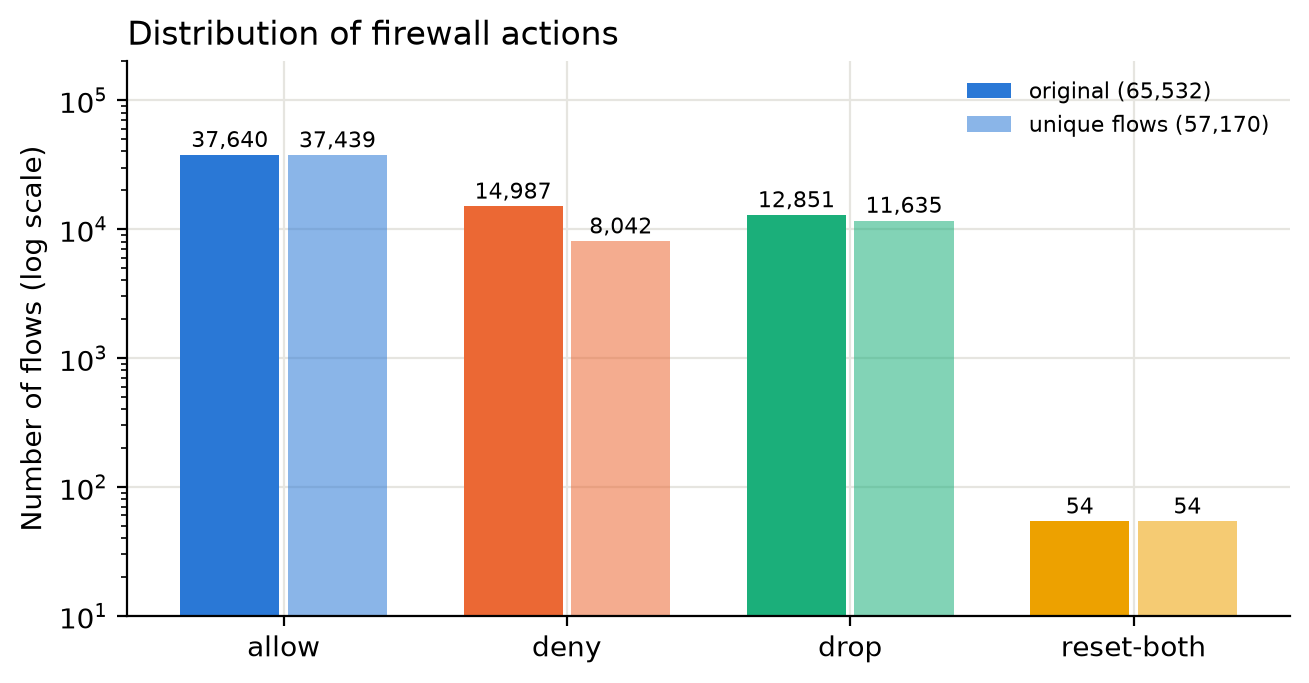
\includegraphics[width=0.8\linewidth,keepaspectratio]{ch03/class_distribution}
  \caption{Distribution of firewall actions before and after deduplication (logarithmic scale)}
  \label{fig:class-distribution}
\end{figure}

This imbalance has two consequences. First, accuracy is a misleading metric: a classifier that always answers \emph{allow} is right 57\,\% of the time. Second, with only 43 \emph{reset-both} examples left for training after the split, this class is very hard to learn; the evaluation must report it separately.

\subsection{Skewness of the volume and duration features}
The volume features are extremely right-skewed (Figure~\ref{fig:skewness}): most flows are tiny (median of 193~bytes and 2~packets on the unique records), while a few transfers reach more than one gigabyte. On the unique records the skewness coefficient is 174.9 for \emph{Bytes}, 148.4 for \emph{Packets} and 11.7 for \emph{Elapsed Time}. Such distributions are dominated by a few extreme values, which would distort distance-based models (\ac{KNN}, \ac{SVM}).

\begin{figure}[htbp]
  \centering
  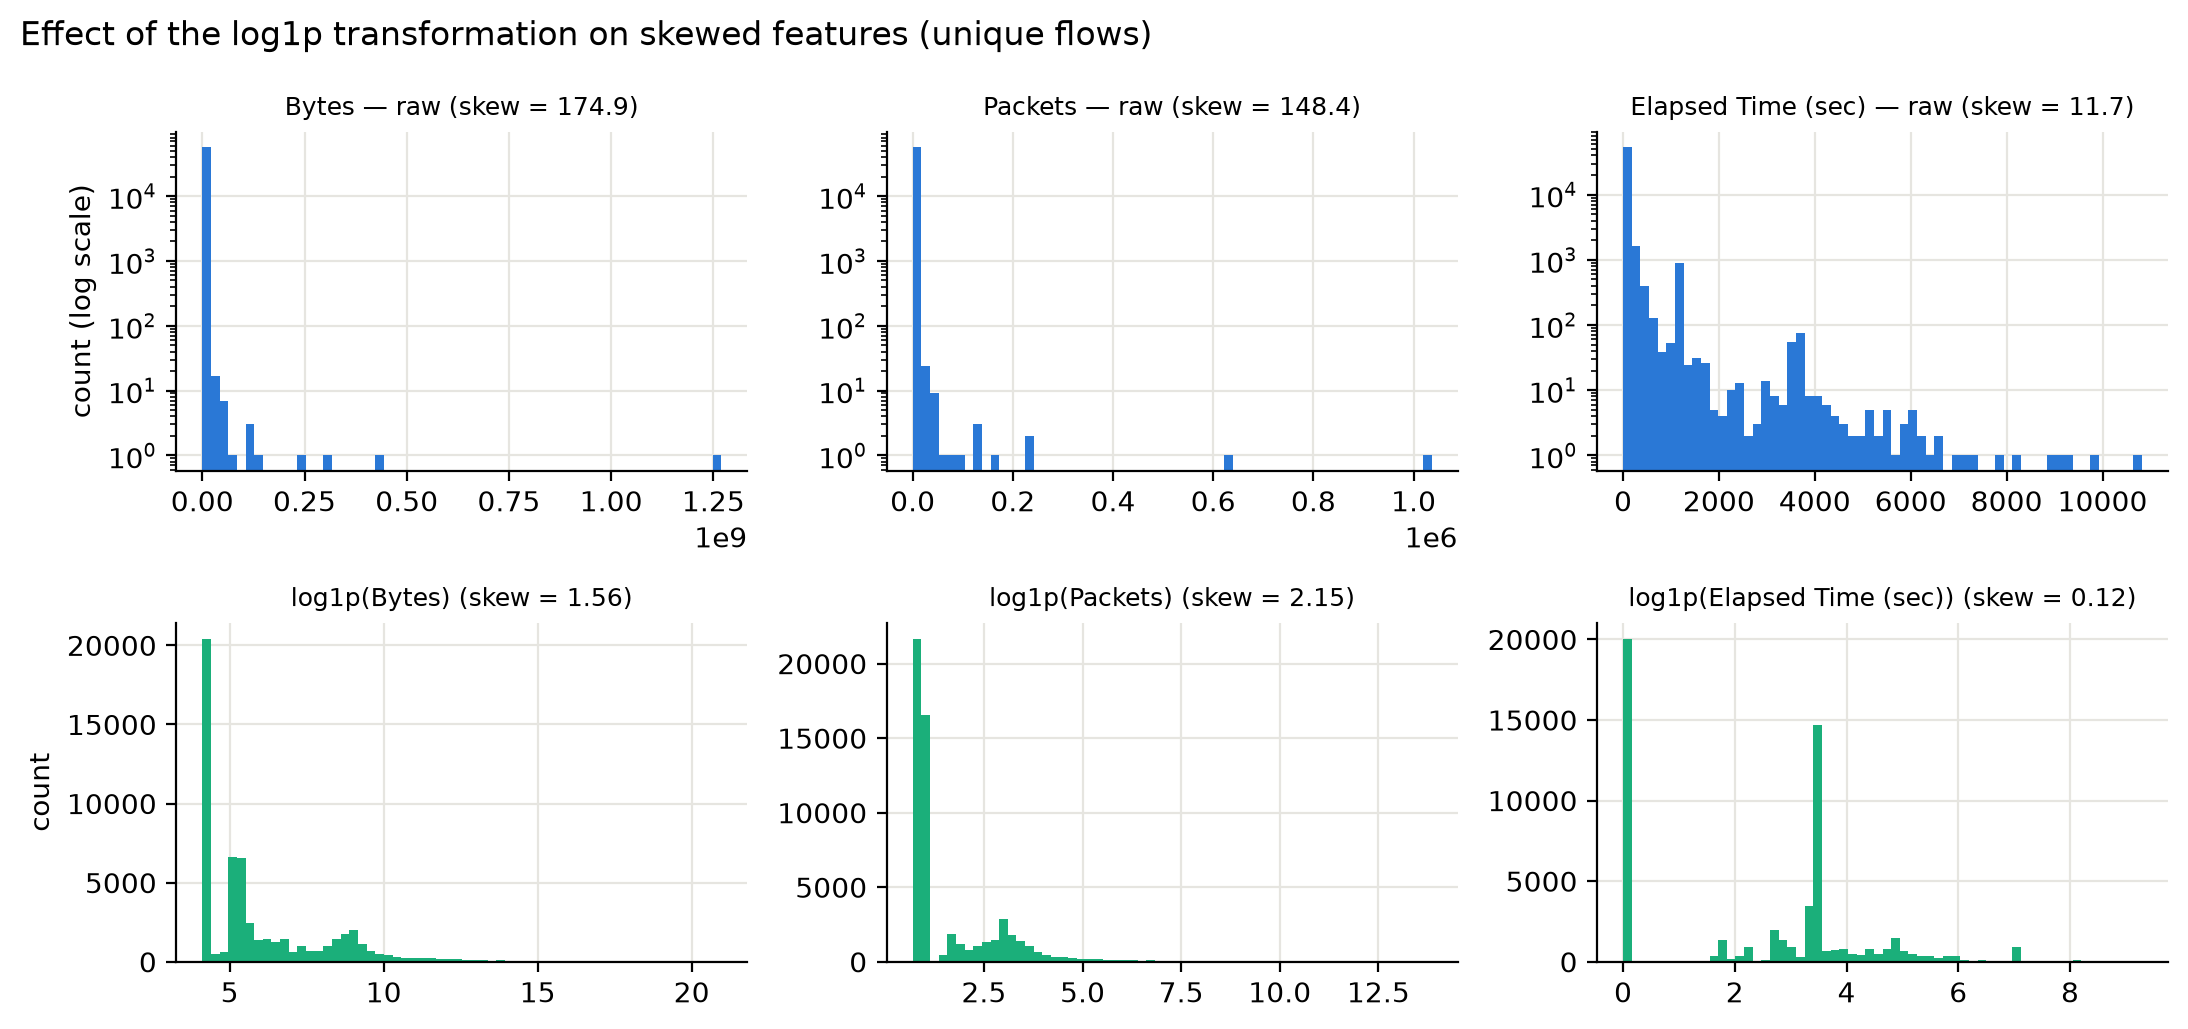
\includegraphics[width=\linewidth,keepaspectratio]{ch03/skewness_log_transform}
  \caption{Distribution of three features before (top) and after (bottom) the $\log(1+x)$ transformation}
  \label{fig:skewness}
\end{figure}

The transformation $x \mapsto \log(1+x)$ compresses the large values while keeping zero at zero; it reduces the skewness to 1.56 for \emph{Bytes}, 2.15 for \emph{Packets} and 0.12 for \emph{Elapsed Time} (bottom row of Figure~\ref{fig:skewness}). The extreme values are \emph{not} removed: they are genuine large transfers, not measurement errors, and after the logarithm they no longer dominate the scale. The transformation is applied inside the model pipeline (Section~\ref{sec:preprocessing}).

\section{Bivariate Analysis and Correlations}
\subsection{Volume and duration by action}
Figure~\ref{fig:boxplots} compares the distributions of volume and duration across the actions. Allowed flows are clearly different: their median duration is 30~seconds and their median volume 422~bytes, whereas \emph{deny}, \emph{drop} and \emph{reset-both} flows have a median duration of 0~seconds and a median of a single packet. The three blocking actions close the connection almost immediately and are much harder to tell apart with these features; \emph{reset-both} flows carry somewhat more bytes (median 145) than \emph{deny} (66) and \emph{drop} (70) flows.

\begin{figure}[htbp]
  \centering
  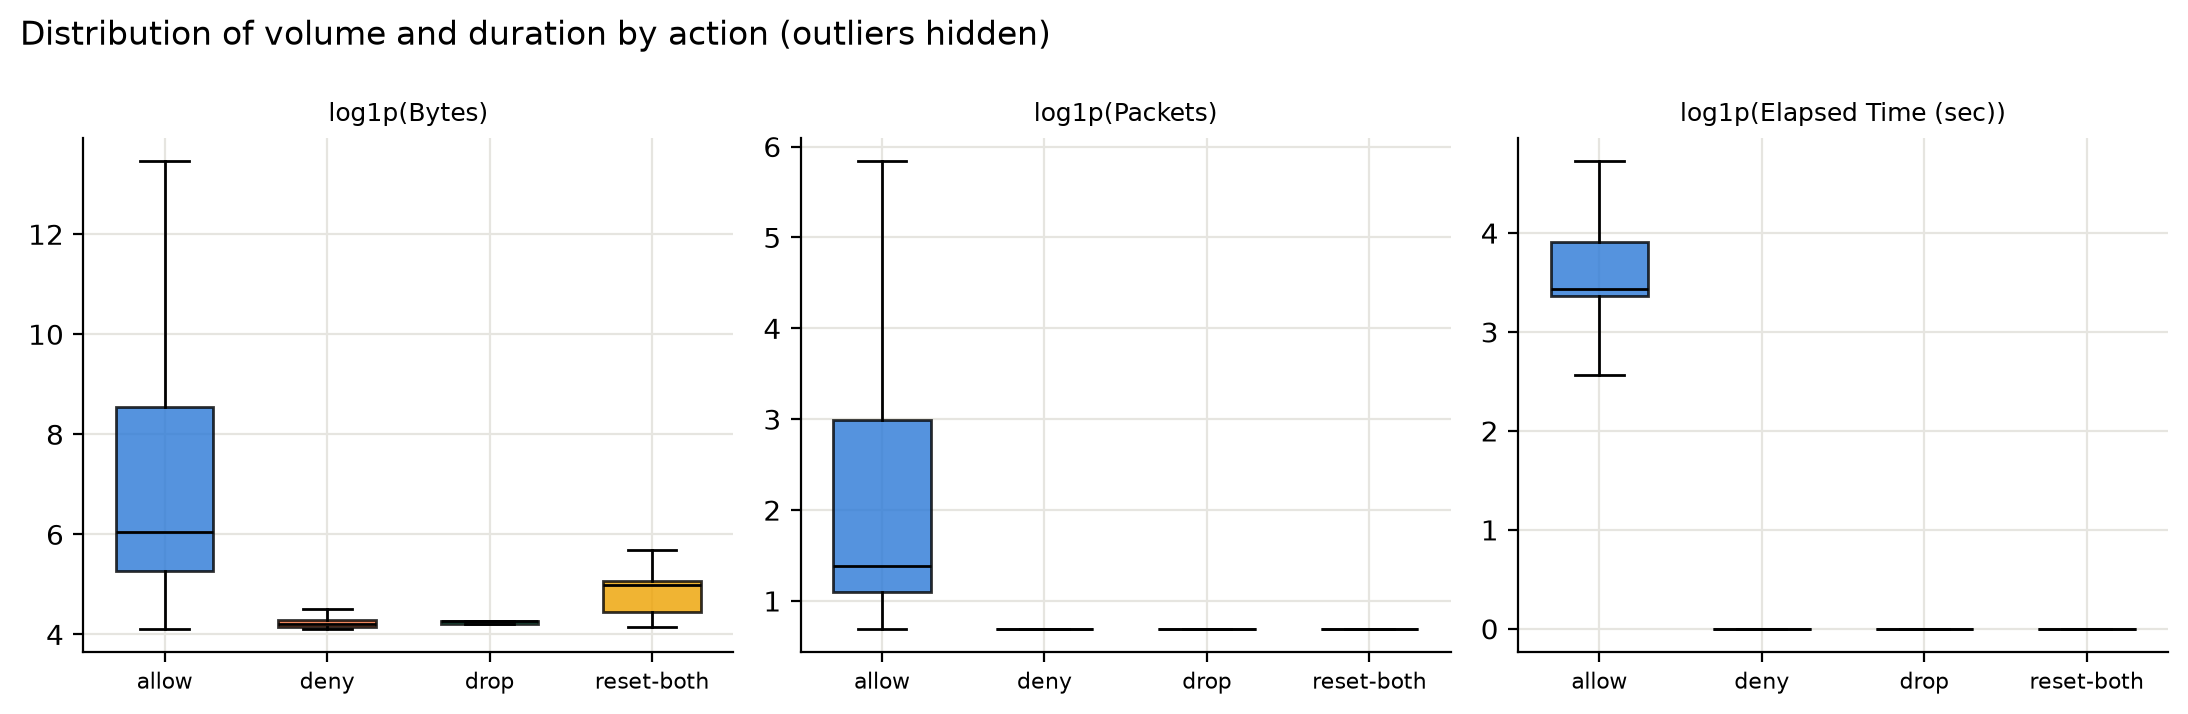
\includegraphics[width=\linewidth,keepaspectratio]{ch03/boxplots_by_action}
  \caption{Volume and duration by action, on the $\log(1+x)$ scale}
  \label{fig:boxplots}
\end{figure}

\subsection{Correlations between numerical features}
Because the features are skewed and not normal (Section~\ref{sec:tests}), the monotonic association between them is measured with the Spearman rank correlation coefficient $\rho$~\cite{spearman1904proof} rather than Pearson's $r$. Figure~\ref{fig:spearman} shows the matrix. The volume features form a block of almost collinear variables: $\rho = 0.98$ between \emph{Bytes Received} and \emph{pkts\_received}, $0.97$ between \emph{Packets} and \emph{pkts\_received}, $0.95$ between \emph{Bytes} and \emph{Bytes Sent}. All 21 coefficients remain significant after Benjamini--Hochberg correction~\cite{benjamini1995controlling}. In practice the seven numerical features carry little more information than two or three of them, which explains why several of them receive a near-zero permutation importance in Chapter~\ref{chap:resultats}.

\begin{figure}[htbp]
  \centering
  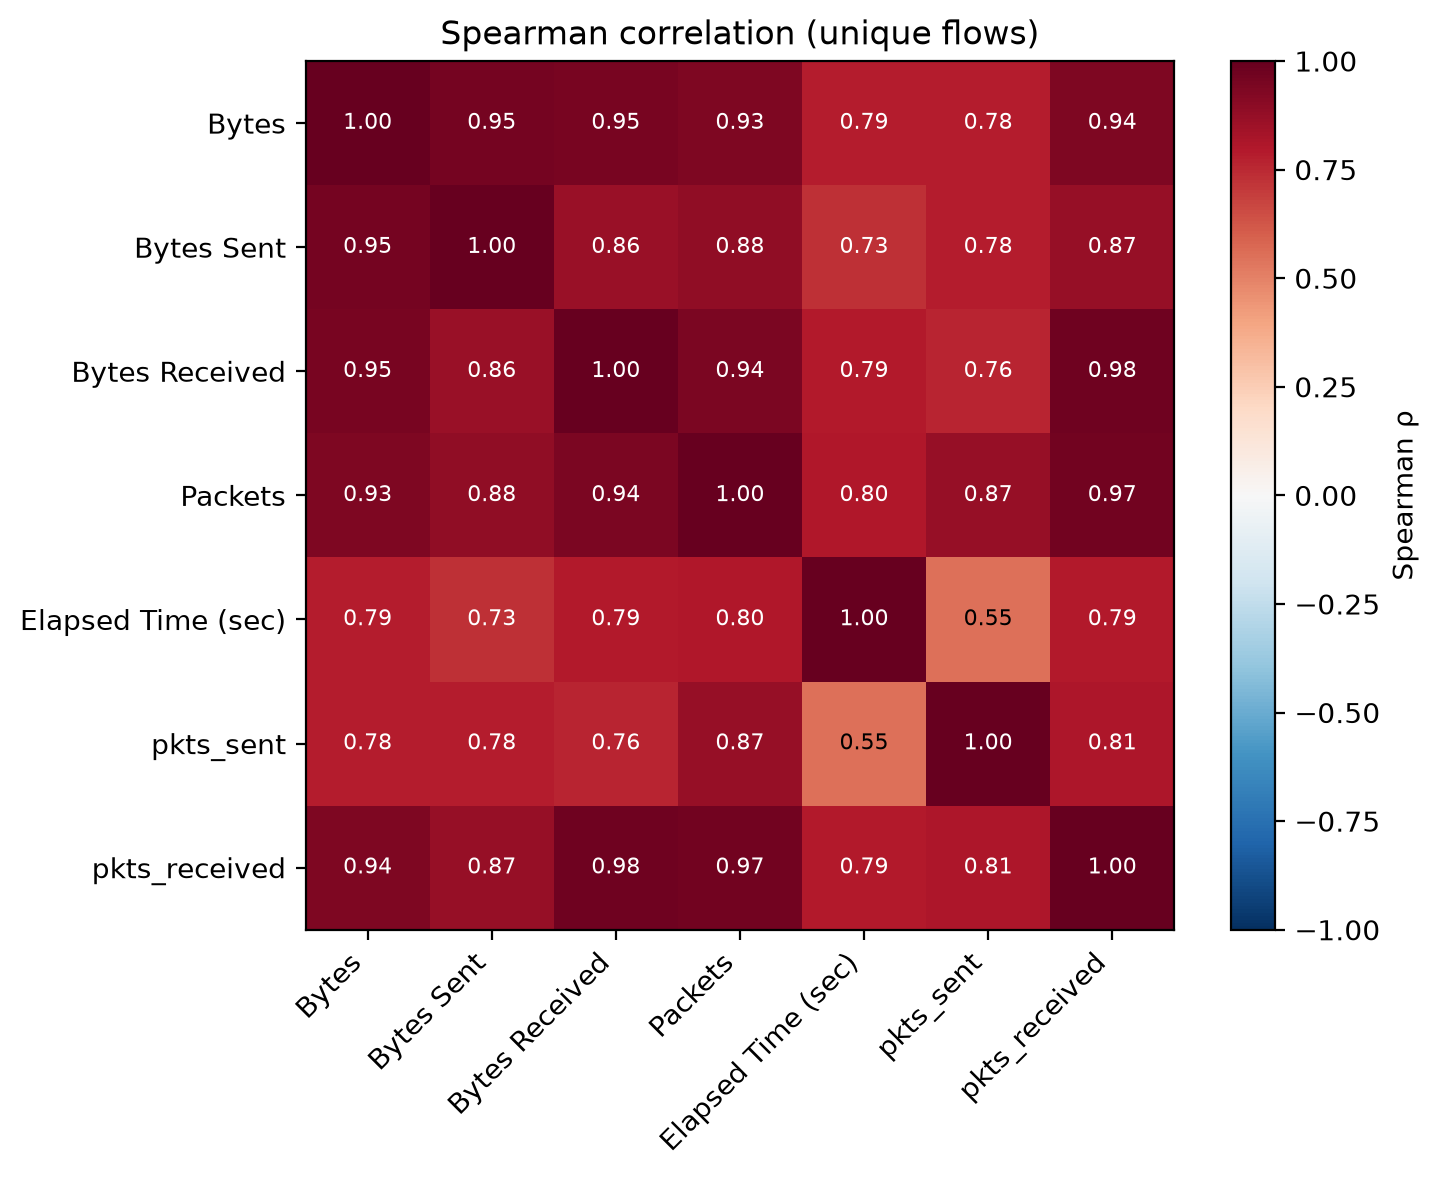
\includegraphics[width=0.62\linewidth,keepaspectratio]{ch03/spearman_heatmap}
  \caption{Spearman correlation matrix of the numerical features (unique records)}
  \label{fig:spearman}
\end{figure}

\subsection{Destination ports: policy signatures}
Destination ports reveal the firewall policy most directly (Figure~\ref{fig:ports}). Port 53 (DNS), 443 (HTTPS) and 80 (HTTP) are almost always allowed; port 445 (SMB, a classic target of worms and ransomware) is dropped in 11\,635 of 11\,674 flows; port 23 (Telnet) and a set of high ports are mostly denied. The \emph{reset-both} flows do not belong to any frequent port: all 54 fall in the ``other'' category, spread over many rare ports (the most common, port 3389 used by remote desktop, accounts for only 12 of them), which already suggests why they are hard to predict.

\begin{figure}[htbp]
  \centering
  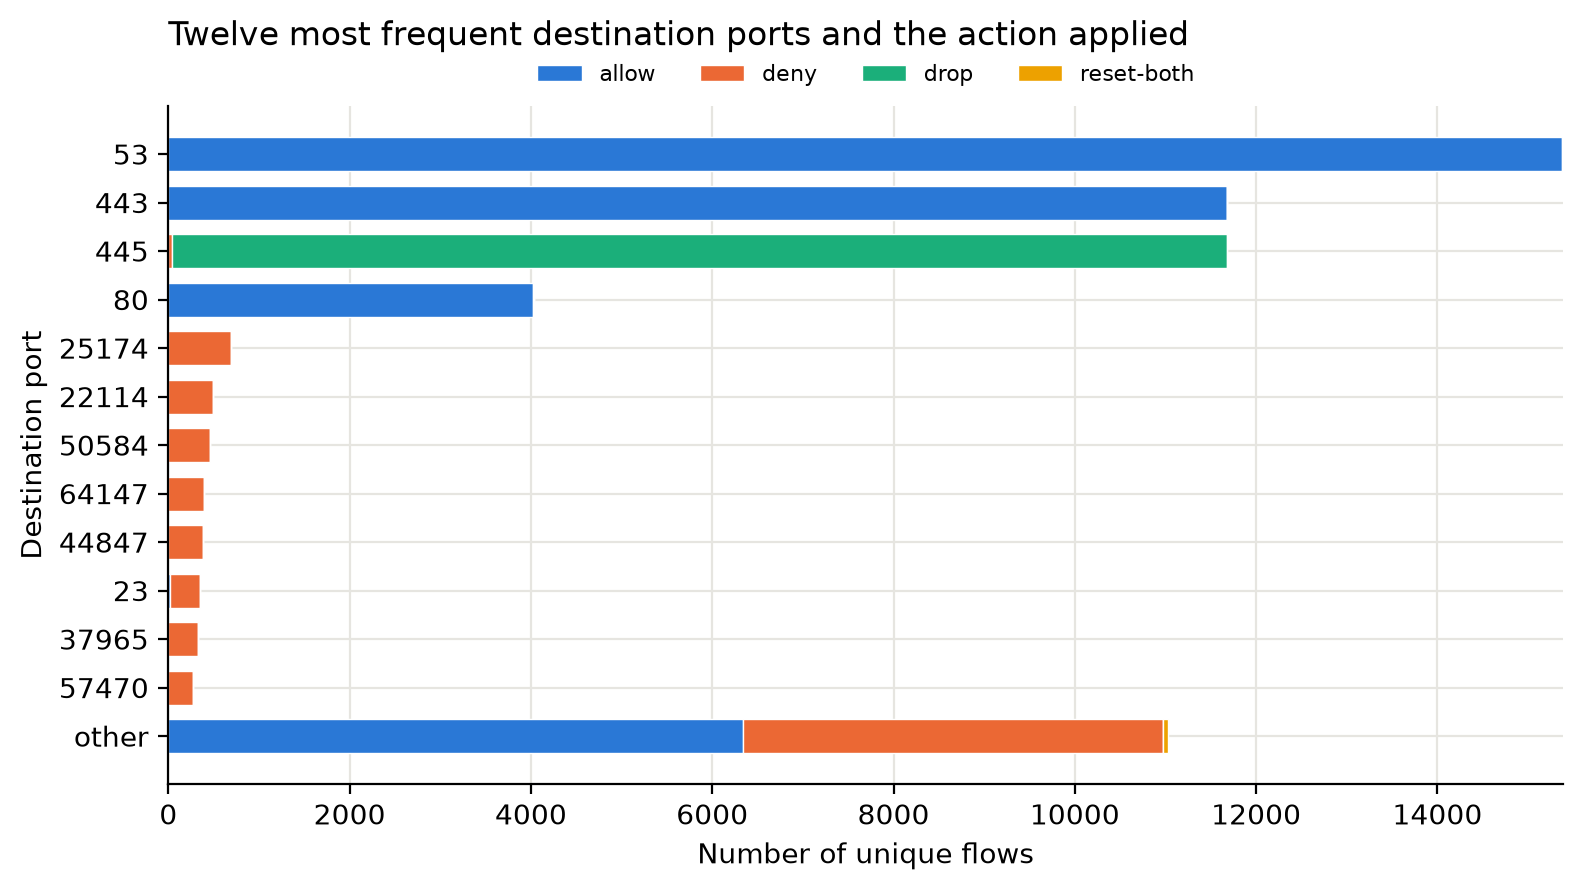
\includegraphics[width=0.9\linewidth,keepaspectratio]{ch03/destination_ports_by_action}
  \caption{Action applied to the twelve most frequent destination ports (unique records)}
  \label{fig:ports}
\end{figure}

\subsection{Network address translation}
Figure~\ref{fig:nat} shows that a non-zero \ac{NAT} source port is almost a signature of allowed traffic: 98.9\,\% of allowed flows are translated, against 0.15\,\% of denied flows and none of the dropped flows. This is plausible network behaviour (a translation is only created for a connection that the firewall lets through), but it also means that the \ac{NAT} fields may be \emph{consequences} of the decision rather than causes. This risk of target leakage is analysed in Chapter~\ref{chap:methodologie}.

\begin{figure}[htbp]
  \centering
  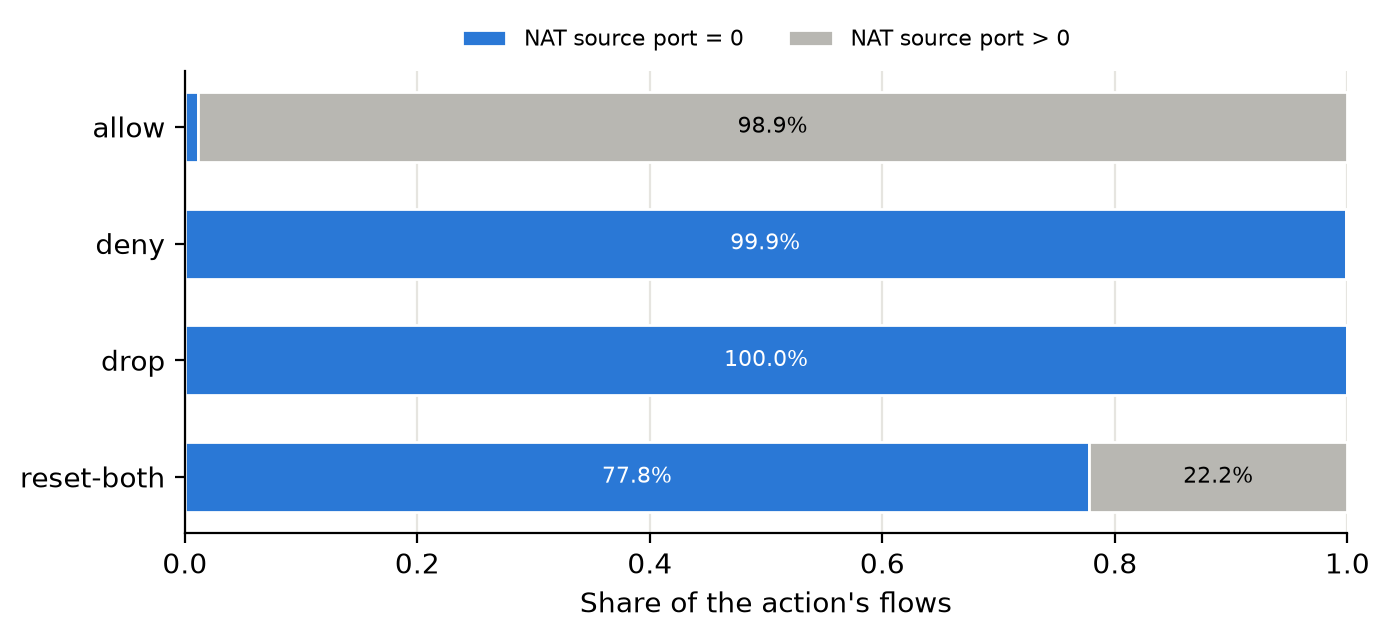
\includegraphics[width=0.75\linewidth,keepaspectratio]{ch03/nat_status_by_action}
  \caption{Share of flows with a translated (non-zero) NAT source port, by action}
  \label{fig:nat}
\end{figure}

\section{Statistical Tests}\label{sec:tests}
The visual observations above are now tested formally. All tests are run on the 57\,170 unique records, because duplicated records violate the independence assumption shared by every test; the results on the original data are reported as a sensitivity check. With $n \approx 57\,000$, almost any difference is statistically significant, so each test is accompanied by an \textbf{effect size}, which carries the practical conclusion. When the computed p-value is smaller than the smallest representable number, it is reported as $p < 10^{-300}$.

\subsection{Test 1 --- Checking the assumptions of ANOVA}
\textbf{Question.} The natural test to compare a numerical feature across four groups is the one-way analysis of variance (ANOVA), which assumes that the feature is normally distributed with the same variance in every group. Are these assumptions met?

\textbf{Tests and justification.} Normality is tested in each group with the Shapiro--Wilk test~\cite{shapiro1965analysis} (on a random sample of at most 5\,000 records per group, the range in which it is reliable) and the D'Agostino--Pearson $K^2$ test~\cite{dagostino1973tests} (on all records). Equality of variances is tested with the Brown--Forsythe test~\cite{brown1974robust}, a version of Levene's test centred on the median that remains valid when the data are not normal. The tests are applied to $\log(1+\text{Bytes})$, that is, after the transformation used by the models: if even the transformed data are not normal, the raw data certainly are not.

\begin{table}[htbp]
  \centering
  \caption{Normality tests on $\log(1+\text{Bytes})$ by action (unique records)}
  \label{tab:normality}
  \begin{tabular}{|l|r|r|r|r|}
    \hline
    \textbf{Action} & $n$ & \textbf{Skewness} & \textbf{Shapiro--Wilk $W$} & \textbf{p-value} \\
    \hline
    allow & 37\,439 & 1.26 & 0.880 & $2.5 \times 10^{-52}$ \\
    deny & 8\,042 & 2.68 & 0.590 & $6.5 \times 10^{-76}$ \\
    drop & 11\,635 & $-0.58$ & 0.610 & $7.4 \times 10^{-75}$ \\
    reset-both & 54 & $-0.17$ & 0.828 & $2.1 \times 10^{-6}$ \\
    \hline
  \end{tabular}
\end{table}

\textbf{Result.} Shapiro--Wilk rejects normality in all four groups (Table~\ref{tab:normality}). The $K^2$ test does not reject it for \emph{reset-both} ($p = 0.074$), where 54 observations give it little power, but the Q--Q plots of Figure~\ref{fig:qq} show the departure clearly: the transformed data form steps and plateaus instead of following the line. The Brown--Forsythe test also rejects equal variances ($W = 6\,217$, $p < 10^{-300}$). \textbf{Conclusion:} ANOVA is not valid for these data, and rank-based (non-parametric) tests are used in the rest of the analysis.

\begin{figure}[htbp]
  \centering
  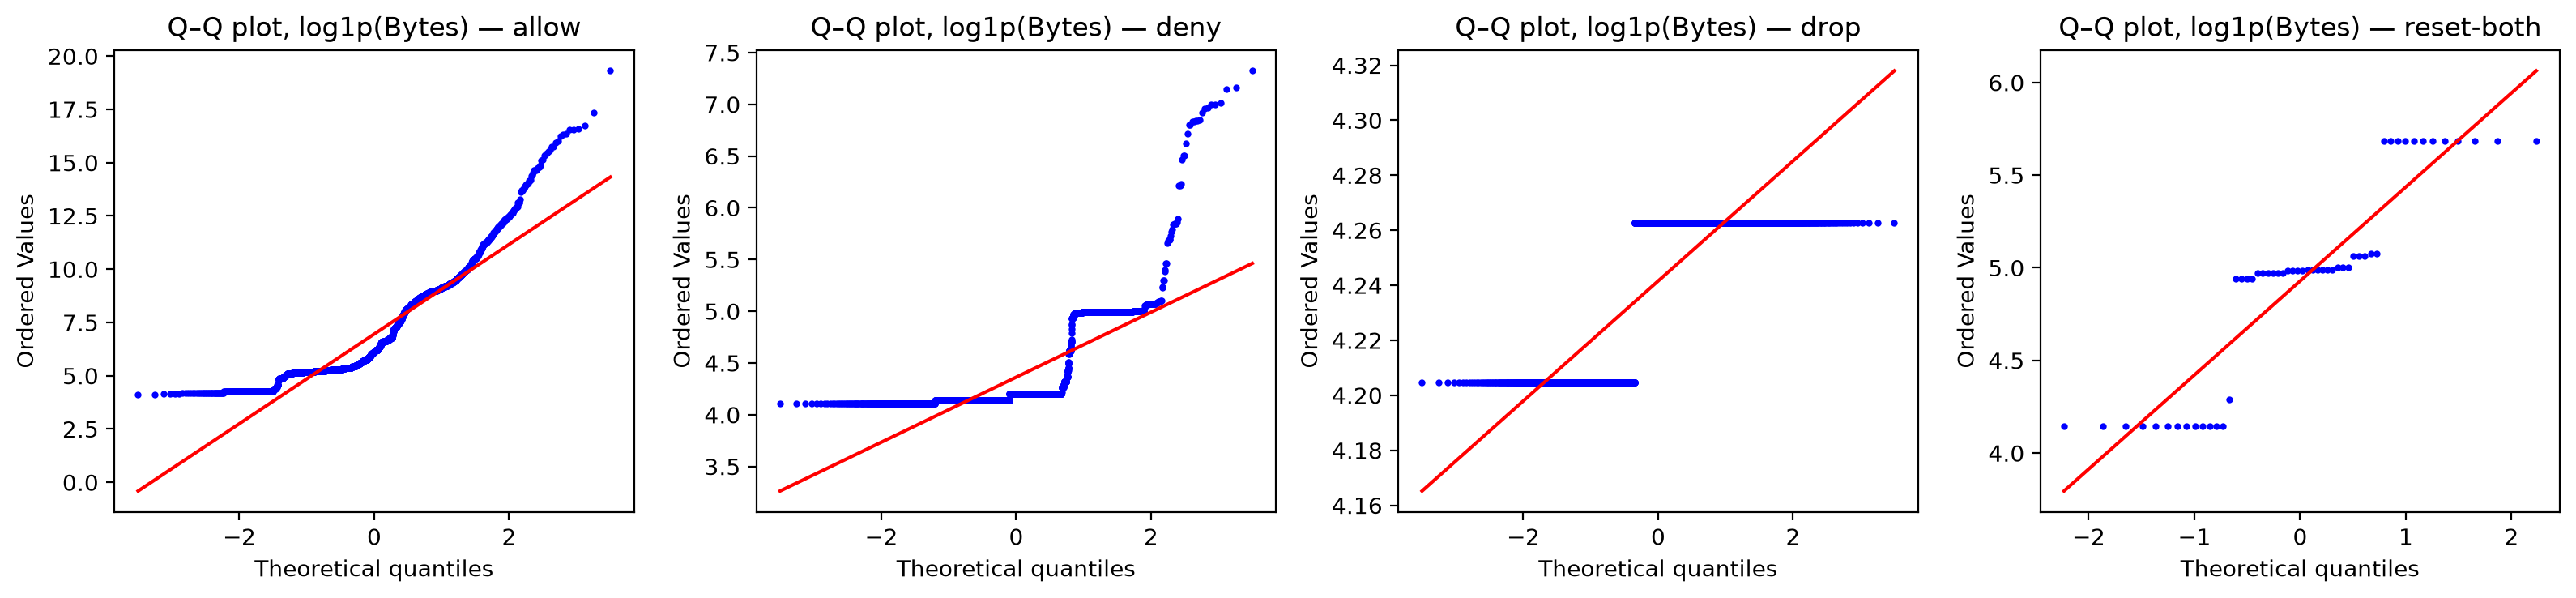
\includegraphics[width=\linewidth,keepaspectratio]{ch03/qq_plots_log_bytes}
  \caption{Normal Q--Q plots of $\log(1+\text{Bytes})$ for each action}
  \label{fig:qq}
\end{figure}

\subsection{Test 2 --- Kruskal--Wallis test on every numerical feature}
\textbf{Question.} Does each numerical feature differ between the four actions?

\textbf{Hypotheses.} $H_0$: the four actions come from the same distribution; $H_1$: at least one action differs.

\textbf{Justification.} The Kruskal--Wallis $H$ test~\cite{kruskal1952use} is the non-parametric counterpart of one-way ANOVA: it compares the mean ranks of $k$ independent groups and needs neither normality nor equal variances. Its effect size is $\varepsilon^2 = H/(n-1)$, interpreted as small around 0.01, medium around 0.08 and large above 0.26. Because seven features are tested, the p-values are adjusted with the Benjamini--Hochberg procedure~\cite{benjamini1995controlling}, which controls the false discovery rate.

\begin{table}[htbp]
  \centering
  \caption{Kruskal--Wallis test of each numerical feature across the four actions (df = 3)}
  \label{tab:kruskal}
  \begin{tabular}{|l|r|r|r|r|}
    \hline
    & \multicolumn{2}{c|}{\textbf{Unique records}} & \multicolumn{2}{c|}{\textbf{Original records}} \\
    \textbf{Feature} & $H$ & $\varepsilon^2$ & $H$ & $\varepsilon^2$ \\
    \hline
    Elapsed Time (sec) & 40\,093 & 0.701 & 51\,428 & 0.785 \\
    Packets & 37\,713 & 0.660 & 48\,398 & 0.739 \\
    Bytes & 34\,771 & 0.608 & 44\,288 & 0.676 \\
    pkts\_received & 34\,694 & 0.607 & 44\,703 & 0.682 \\
    Bytes Received & 33\,879 & 0.593 & 43\,965 & 0.671 \\
    Bytes Sent & 28\,533 & 0.499 & 37\,074 & 0.566 \\
    pkts\_sent & 15\,323 & 0.268 & 20\,655 & 0.315 \\
    \hline
  \end{tabular}
\end{table}

\textbf{Result.} $H_0$ is rejected for all seven features ($p < 10^{-300}$ after correction), with large effect sizes (Table~\ref{tab:kruskal}). Duration and packet counts separate the actions best. The effects are slightly smaller on unique records than on the original data, which shows that the duplicates artificially inflate the apparent separation.

\subsection{Test 3 --- Dunn post-hoc test: which actions differ?}
\textbf{Question.} The Kruskal--Wallis test only states that \emph{at least one} action differs. Which pairs of actions actually differ?

\textbf{Justification.} Dunn's test~\cite{dunn1964multiple} compares every pair of groups using the joint ranks of the Kruskal--Wallis test (with a correction for ties). Six pairs are compared for each feature, so the p-values are adjusted with Holm's method~\cite{holm1979simple}. The size and direction of each difference are measured with Cliff's $\delta$~\cite{cliff1993dominance}, the probability that a value of the first group exceeds a value of the second minus the reverse probability ($|\delta| < 0.147$ negligible, $< 0.33$ small, $< 0.474$ medium, otherwise large).

\begin{table}[htbp]
  \centering
  \caption{Dunn post-hoc test (Holm-adjusted p-values) and Cliff's $\delta$, unique records}
  \label{tab:dunn}
  \small
  \begin{tabular}{|l|r|r|r|r|r|r|}
    \hline
    & \multicolumn{2}{c|}{\textbf{Bytes}} & \multicolumn{2}{c|}{\textbf{Packets}} & \multicolumn{2}{c|}{\textbf{Elapsed Time}} \\
    \textbf{Pair} & $p_{\text{Holm}}$ & $\delta$ & $p_{\text{Holm}}$ & $\delta$ & $p_{\text{Holm}}$ & $\delta$ \\
    \hline
    allow vs deny & $<10^{-300}$ & $+0.93$ & $<10^{-300}$ & $+0.95$ & $<10^{-300}$ & $+0.99$ \\
    allow vs drop & $<10^{-300}$ & $+0.95$ & $<10^{-300}$ & $+0.95$ & $<10^{-300}$ & $+0.99$ \\
    allow vs reset-both & $2.1\times10^{-14}$ & $+0.71$ & $3.3\times10^{-21}$ & $+0.72$ & $2.1\times10^{-34}$ & $+0.99$ \\
    deny vs drop & $4.8\times10^{-49}$ & $-0.38$ & 0.86 & $0.00$ & 1.00 & $0.00$ \\
    deny vs reset-both & $5.2\times10^{-7}$ & $-0.50$ & 0.009 & $-0.22$ & 1.00 & $-0.13$ \\
    drop vs reset-both & $3\times10^{-4}$ & $-0.52$ & 0.009 & $-0.22$ & 1.00 & $-0.13$ \\
    \hline
  \end{tabular}
\end{table}

\textbf{Result.} Table~\ref{tab:dunn} gives a precise picture of the problem:
\begin{itemize}
  \item every pair involving \emph{allow} differs with a large effect: allowed flows are longer and larger;
  \item \textbf{duration does not separate the three blocking actions at all} ($p_{\text{Holm}} = 1$, negligible $\delta$): \emph{deny}, \emph{drop} and \emph{reset-both} all end immediately;
  \item \emph{deny} and \emph{drop} differ on volume (medium effect) but not on packets or duration; the destination port separates them much better (Test~4);
  \item \emph{reset-both} carries more bytes than \emph{deny} with a large effect ($\delta = -0.50$), but this difference rests on only 54 flows whose distribution overlaps strongly with \emph{deny}.
\end{itemize}
These results provide the statistical explanation of the main limitation found in Chapter~\ref{chap:resultats}: classifiers confuse \emph{reset-both} with \emph{deny}.

\subsection{Test 4 --- Chi-square tests of independence}
\textbf{Question.} Are the categorical attributes, \ac{NAT} status and destination port, associated with the action?

\textbf{Hypotheses.} $H_0$: the attribute and the action are independent; $H_1$: they are associated.

\textbf{Justification.} Both variables are categorical, so Pearson's $\chi^2$ test of independence on the contingency table is appropriate. It is valid when every expected count is at least 5 (Cochran's rule), which is checked. The strength of the association is measured with Cramér's $V$~\cite{cramer1946mathematical}, between 0 (independence) and 1 (perfect association).

\textbf{Result (a) --- NAT source-port status} (zero / non-zero) $\times$ action: $\chi^2 = 55\,264$, df $= 3$, $p < 10^{-300}$, $V = 0.98$; the smallest expected count is 19.0, so the test is valid. On the original data, $\chi^2 = 63\,183$ and $V = 0.98$. The association is almost perfect, which confirms Figure~\ref{fig:nat}.

\textbf{Result (b) --- destination port} (ten most frequent ports plus ``other'') $\times$ action: $\chi^2 = 88\,899$, df $= 30$, $V = 0.72$. Here seven expected counts are below 5 (in the rare \emph{reset-both} column), so the asymptotic p-value is not reliable. A \textbf{Monte Carlo permutation test} was used instead: the action labels were shuffled 999 times and $\chi^2$ recomputed each time. The largest value obtained under $H_0$ was 69, far below the observed 88\,899, giving $p = 1/1000 = 0.001$, the smallest value attainable with 999 permutations. The destination port is therefore strongly associated with the action, consistent with port-based firewall rules.

\section{Summary and Identified Risks}
The exploration shows that the problem is largely separable: the destination port, the duration and the volume of a flow differ strongly between actions, with large effect sizes. It also identifies four risks that the methodology must handle. The first is \textbf{class imbalance}: \emph{reset-both} represents 0.08\,\% of the data, so accuracy is misleading and per-class results must be reported. The second is \textbf{duplicates}: 12.8\,\% of the records are copies, which would inflate the scores if copies were split between training and test sets. The third is \textbf{redundancy}: totals equal the sum of their components and the volume features are almost collinear. The last is \textbf{possible target leakage}: the \ac{NAT} fields and the flow duration may only be known after the firewall's decision.

\section{Conclusion}
This chapter described a clean but highly imbalanced data set, in which ports act as policy signatures and the volume features are skewed and redundant. Five statistical tests, each chosen after checking its assumptions, confirmed that the actions differ strongly on most features, but that the three blocking actions are hard to separate by duration and that \emph{reset-both} overlaps with \emph{deny}. Chapter~\ref{chap:methodologie} builds on these findings to design a preprocessing pipeline and an evaluation protocol that control duplicates, skewness and leakage.
